\documentclass[12pt,a4paper, titlepage, openany]{book}
\usepackage{amsmath}
\usepackage{graphicx}
\usepackage{float}
\usepackage{wrapfig}
\usepackage[russian]{babel}
\usepackage[utf8]{inputenc}
\usepackage{geometry}
\usepackage{hyperref}
\geometry{left = 5cm}
\geometry{right = 2cm}
\hypersetup{
	colorlinks=true,
	linkcolor=red,
	linktocpage=true
}


\hoffset = 0pt
\voffset = 0pt
\textheight = 700pt
\topmargin = 0pt
\headheight = 0pt
\headsep = 15pt
\marginparwidth = 0pt
\oddsidemargin = 0pt
\textwidth = 450pt
\setcounter{tocdepth}{3}

\begin{document}
\begin{titlepage}
\newpage
\centerline{\footnotesize{Федеральное государственное автономное образовательное учреждение высшего образования}}
\centerline{\footnotesize{<<Московский физико-технический институт (национальный исследовательский университет)>>}}
\centerline{\footnotesize{Физтех-школа Аэрокосмических Технологий}}
\centerline{\footnotesize{Кафедра вычислительной физики}}
\hfill \break

\centerline{\footnotesize{\textbf{Направление подготовки / специальность:} 03.03.01 Прикладные математика и физика}}
\centerline{\footnotesize{\textbf{Направленность (профиль) подготовки:} Геокосмические науки и технологии}}

\hfill \break
\hfill \break
\hfill \break
\begin{center}
\Large{\textbf{Численное решение задач,
 описывающих динамическое поведение ледовых структур}}
\end{center}
\hfill \break
\centerline{(бакалаврская работа)}
\hfill \break

\small{
\begin{flushright}
\begin{minipage}{.40\textwidth}
\textbf{Студент:}\\
Петраков Иван Николаевич\\
\hfill \break
\underline{\hspace{6cm}}\\
\centerline{\footnotesize{\textit{(подпись студента)}}}\\
\hfill \break
\textbf{Научный руководитель:}\\
Петров Игорь Борисович,\\
д-р физ.-мат. наук, проф., чл.-кор. РАН
\hfill \break
\hfill \break
\underline{\hspace{6cm}}\\
\centerline{\footnotesize{\textit{(подпись научного руководителя)}}}\\
\hfill \break
\textbf{Консультант:}\\
Иванов Иван Иванович\\
\hfill \break
\underline{\hspace{6cm}}\\
\centerline{\footnotesize{\textit{(подпись консультанта)}}}\\
\end{minipage}
\end{flushright}
}
\hfill \break
\hfill \break
\centerline{Долгопрудный - 2022}
\end{titlepage}


\tableofcontents

\chapter{Введение}


\chapter{Модель среды}
В данной главе описывается модель среды, которая используется в работе.



\section{Линейно-упругая среда}
\par
Для описания определенных процессов в природе (например, волновых процессов в упругой среде) используется линейная теория упругости, в основе которой лежат два уравнения для описания движения бесконечно-малого объема линейно-упругой среды.
\par
Первое уравнение - уравнение движения:
\begin{equation}
\rho \frac{\partial v_i}{\partial t} = \frac{\partial \sigma_{ij}}{\partial x_j}
\end{equation}
где $\rho$ - плотность среды, $v_i$ - компоненты скорости среды в точке, $\sigma_{ij}$ - тензор напряжений Коши.
\par
Второе уравнение - реологическое соотношение между деформациями и напряжениями:
\begin{equation}
\label{eq:2.2}
\begin{aligned}
e_{ij} &= \frac{1}{2}(\frac{\partial u_i}{\partial x_j} + \frac{\partial u_j}{\partial x_i}),\\
\sigma_{ij} &= C_{ijkl} e_{kl}
\end{aligned}
\end{equation}
где $u_i$ - вектор смещения точки тела, $C_{ijkl}$ - тензор упругости, $e_{ij}$ - тензор деформаций.
\par
Для линейно-упругой среды тензор упругости зависит только от двух независимых величин $\lambda$ и $\mu$, которые называются параметрами Ламе. Тогда \ref{eq:2.2} можно переписать в виде:
\begin{equation}
\label{eq:2.3}
\sigma_{ij} = \lambda \delta_{ij} e_{kk} + 2 \mu e_{ij}
\end{equation}
где $\delta_{ij}$ - символ Кронекера. 
\par
Также можно учесть, что тензор деформаций симметричен в силу закона парности касательных напряжений, поэтому если продифференцировать \ref{eq:2.3} по времени, можно получить окончательную систему определяющих уравнений линейно-упругой среды:
\begin{equation}
\label{eq:2.4}
\begin{cases}
\rho \frac{\partial v_i}{\partial t} = \frac{\partial \sigma_{ij}}{\partial x_j}, \\
\frac{\partial \sigma_{ij}}{\partial t} = \lambda(\frac{\partial}{\partial x_k} v_k) \delta_{ij} + \mu(\frac{\partial v_i}{\partial x_j} + \frac{\partial v_j}{\partial x_i}).
\end{cases}
\end{equation}















\section{Линейно-акустическая среда}
\par
Определяющие уравнения линейно-акустической среды получаются из фундаментальных уравнений гидродинамики (уравнения неразрывности и уравнения Эйлера):
\begin{equation}
\label{eq:2.5}
\begin{aligned}
\frac{\partial \rho}{\partial t} + \nabla \cdot (\rho \mathbf{v}) = \frac{\partial \rho}{\partial t} + \mathbf{v} \cdot \nabla \rho + \rho \nabla \cdot \mathbf{v} &= 0, \\
\frac{\partial \mathbf{v}}{\partial t} + (\mathbf{v} \cdot \nabla) \mathbf{v} + \frac{\nabla p}{\rho} &= 0
\end{aligned}
\end{equation}
где $\rho$ - плотность среды, $\mathbf{v} = (v_x, v_y, v_z)$ - скорость жидкости, $p$ - давление. При этом предполагается, что отклонения плотности, скорости и давления относительно стационарного потока малы:
\begin{equation}
\label{eq:2.6}
\rho = \rho_0 + \rho', \mathbf{v} = \mathbf{v_0} + \mathbf{v'}, p = p_0 + p'
\end{equation}
\par
Считая, что плотность не зависит от координаты, и тот факт, что стационарый поток должен подчиняться закону сохранения массы, получаем, что поле $\mathbf{v_0}$ должно быть соленоидальным, т.е.
\begin{equation}
\label{eq:2.7}
\nabla \cdot \mathbf{v_0} = 0
\end{equation}
\par
Подставляя \ref{eq:2.7} и \ref{eq:2.6} в \ref{eq:2.5} получаем:
\begin{equation}
\frac{\partial \rho '}{\partial t} + \mathbf{v_0} \cdot \nabla \rho' + \rho_0 \nabla \cdot \mathbf{v'} = 0.
\end{equation}
\par
В нашей модели считаем процесс распространения малых возмужений адиабатическим, тогда 
\begin{equation}
p' = c^2_p \rho' 
\end{equation}
где
\begin{equation}
c_p = (\frac{\partial p}{\partial \rho})_S
\end{equation}
$S$ - энтропия, $c^2_p = \frac{K}{\rho} = \frac{\lambda}{\rho}$ - скорость акустических волн. Здесь мы воспользовались тем, что в идеальной жидкости нет сдвиговых напряжений и $\mu$ = 0.
\par
Объединяя предыдущие уравнения, получим:
\begin{equation}
\frac{\partial p '}{\partial t} + \mathbf{v_0} \cdot \nabla p' + \lambda \nabla \cdot \mathbf{v'} = 0.
\end{equation}
\par
Осталось получить уравнения для производной по времени малых изменений скорости. Проводим аналогичные действия и получаем:
\begin{equation}
\frac{\partial \mathbf{v'}}{\partial t} + (\mathbf{v_0} \cdot \nabla) \mathbf{v'} + \frac{\nabla p'}{\rho_0} = 0
\end{equation}
\par
Используя связь между нормальными напряжениями и давлением 
\begin{equation}
\sigma_{xx} = \sigma_{yy} = \sigma_{zz} = -p'
\end{equation}
получим итоговую систему для акустоупругой системы в тензорном представлении:
\begin{equation}
\begin{cases}
\rho \frac{\partial v_i}{\partial t} + v^0_k \frac{\partial v_i}{\partial x_k} = \frac{\partial \sigma_{ij}}{\partial x_i}, \\
\frac{\partial \sigma_{ij}}{\partial t} + v^0_k \frac{\partial \sigma_{ij}}{\partial x_k} = \lambda \frac{\partial  v_k}{\partial x_k} \delta_{ij} + \mu (\frac{\partial v_i}{\partial x_j} + \frac{\partial v_j}{\partial x_i})
\end{cases}
\end{equation}
где для акустической системы  $\mu = 0, \mathbf{v_0} \neq 0$, а для упругой - $\mu \neq 0, \mathbf{v_0} =  0$.









\section{Упруго-пластическая среда}
\label{sec:2.3}
\subsection{Основные положения}
Ниже пойдет речь о классической модели упругопластичности, используемой в работе. Рассмотрение ведем в изотермическом приближении.
\par
Характерными особенностями упругопластического поведения являются:
\begin{enumerate}
\item существование диапазона нагрузок, при которых тело ведет себя упруго,
\item существование критерия пластичности (предела текучести), то есть условия, при выполнении которого движение среды происходит по иным законам,
\item отсутствие влияния темпа деформации на возникающие напряжения.
\end{enumerate}
\par
Основными определяющими физическими величинами в теории упруго-пластической среды являются введенные в первой секции главы тензоры напряжений и деформаций. Тензор деформаций складывается из упругой $e_e$ и пластической $e_p$ деформаций. В трехмерном варианте обозначаем тензор деформаций за $\mathbf{E}$.
\par
В качестве критерия пластичности часто задают функцию текучести, которая может зависить как от тензора напряжений $\mathbf{T}$, так и от накопленных пластических деформаций и, возможно, от дополнительных параметров упрочнения $\epsilon$ (причем зависимость от пластических деформаций и параметров упрочнения отсутствует при рассмотрении идеального пластического материала):
\begin{equation}
f(\mathbf{T}, \mathbf{E}_p, \epsilon) = 0
\end{equation}
\par
Рассмотрим идеальный пластический материал, тогда свободная энергия зависит только от упругих деформаций $\psi = \psi(\mathbf{E}_e)$. Определяющее соотношение для тензора напряжений имеет вид (вывод его оставим за кадром):
\begin{equation}
\mathbf{T} = \rho \frac{\partial \psi}{\partial \mathbf{E}_e}
\end{equation}
\par
Неравенство диссипации для пластического течения имеет вид:
\begin{equation}
\mathbf{T}:d\mathbf{E}_p \geq 0
\end{equation}
\par
Положив
\begin{equation}
d\mathbf{E}_p = d \lambda \frac{\partial f}{\partial \mathbf{T}}
\end{equation}
где $d \lambda$ - неопределенный положительный множитель, мы удовлетворим неравенству диссипации. Это выражение называется ассоциированным законом пластического течения.
\subsection{Условия текучести}
Различные модели пластичности основаны на различных функциях текучести. Приведем здесь несколько условий текучести.
\subsubsection{Условие текучести Треска}
Модель Треска предложения для описания пластического поведения металлов. Функция $f$ имеет вид
\begin{equation}
f = \tau - c
\end{equation}
где $\tau$ - максимальное касательное напряжение, $c$ - предел текучести.
\subsubsection{Условие текучести Кулона-Мора}
Для сыпучих сред появляется необходимость учета внутреннего трения, зависящего от нормальных напряжений, поэтому 
\begin{equation}
f = \tau_n - \sigma_n tg \phi - c,
\end{equation}
где $\tau_n$ и $\sigma_n$ - касательное и нормальное напряжения на одной площадке с нормалью $\mathbf{n}$, $c$ - сцепление, $\phi$ - угол внутреннего трения.
\subsubsection{Условие текучести Мизеса}
В модели Мизеса вместо максимального касательного напряжения, как в модели Треска, используется напряжение Мизеса $q = \sqrt{3/2 \mathbf{T'}:\mathbf{T'}} = \sqrt{3 J^{\sigma}_2 (\mathbf{T'})}$, где величина $\sqrt{J^{\sigma}_2 (\mathbf{T'})}$ называется интенсивностью касательных напряжений. Здесь $'$ обозначает девиаторную часть тензора.
\par
Функция f имеет вид
\begin{equation}
f = q - c
\end{equation}
\par
Если учесть тот факт, что интенсивность касательных напряжений пропорциональна энергии формоизменения в упругом теле, то можно сформулировать критерий пластичности Мизеса: \textit{пластическое течение начинается тогда, когда энергия формоизменения достигает критической величины}.
\subsubsection{Условие текучести Друкера-Прагера}
Условие текучести Друкера-Прагера является обобщение условия текучести Мизеса. Функция текучести имеет вид
\begin{equation}
f = q - kp - c
\end{equation}
где $q$ - напряжение по Мизесу, $p$ - давление, $k$ - коэффициент внутреннего трения.
\subsection{Определяющие уравнения}
В настоящей работе используется модель Прандтля-Рейса с условием текучести Мизеса-Шлейхерта (для удобства запишем покомпонентно):
\begin{equation}
\begin{cases}
\rho \dot{v_i} = \nabla_j \sigma_{ij}, \\
\sigma_{ij} = q_{ijkl}e_{kl}
\end{cases}
\end{equation}
где
\begin{equation}
q_{ijkl} = \lambda \delta_{ij}\delta_{kl} + \mu(\delta_{ik}\delta_{jl} + \delta_{il}\delta_{jk}) - \frac{\mu I \sigma_{ij}\sigma_{kl}}{k^2}
\end{equation}
\begin{equation}
\label{eq:2.25}
k = k_0 + \alpha p
\end{equation}
\begin{equation}
\label{eq:2.26}
\begin{cases}
I = 0, s_{ij} : s_{ij} < 2k^2 \\
I = 1, s_{ij} : s_{ij} \geq 2k^2
\end{cases}
\end{equation}
где $k_0$ и $\alpha$ являются параметрами материала, однозначно определяющими $k$ - критерий текучести на сдвиг, $s_{ij}$ - девиатор тензора напряжений, $p$ - давление. Уравнения \ref{eq:2.25} и \ref{eq:2.26} называются условием Мизеса-Шлейхерта.
\par
Стоит отметить, что \ref{eq:2.25} автоматически учитывает упрочнение (зависимость функции текучести от пластических деформаций и параметров упрочнения).







\section{Разрушение. Теория повреждаемости}
Для описания разрушения материала (образования новых поверхностей) существуют две теории: теория прочности и теория повреждаемости,- причем разрушение можно разделить на вязкое (учитываются пластические деформации) и хрупкое (пластические деформации не учитываются). Первая теория (теория прочности) часто дает неправильный результат, потому что не учитываются микротрещины в области трещины. 
\par
В настоящей работе для описания разрушения используется теория повреждаемости, основанная на введении некоторого непрерывного параметра $0 < D < 1$, который называется параметром повреждаемости, отвечающий за изменение эффективной площади с учетом микротрещин.
\par 
Особенности программного учета разрушения будут описаны в следующей главе.



\section{Реология льда}
В настоящей работе рассматривается только морской лед.
\par
Физико-механические свойства льда зависят от температуры и солености, которые меняются по глубине. Некоторые параметры, однако, можно считать постоянными и не зависящими от глубины. Такими являются плотность $\rho$, которая не зависит от давления p в силу большой величины максимального давления и судя по ударной адиабате, и коэффициент Пуассона $\nu = 0.295$, который считается постоянным в широком диапазоне температур (-3.6 ... -15 $^{\circ} C$) и солености (0.113 ... 6.11 \%$_0$). Модуль Юнга зависит только от объема солевого раствора $v_b$:
\begin{equation}
E = E_0(1-v_b)^4
\end{equation}
где объем солевого раствора $v_b$ зависит только от солености $s$ и температуры $T$, которые, в свою очередь, являются функциями вертикальной координаты. В настоящей работе распределение температуры считается линейным от температуры плавления на нижней границы до температуры окружающей среды на верхней. Обьем солевого раствора как функция солености и температуры имеет вид:
\begin{equation}
v_b = s(\frac{49.185}{|T|} + 0.532)
\end{equation}
что справедливо для интервала температур -22.9 ... -0.5 $^{\circ} C$
\par
Лёд можно представить упруго-пластической моделью среды \ref{sec:2.3}. При этом при выполнении некоторого критерия говорится о разрушении материала и последующей эрозии. 
\par
Термическими эффектами в настоящей работе нельзя пренебречь, так как из закономерностей $\frac{dT}{dP} \sim -0.074^{\circ} C$ МПа$^{-1}$ и $\frac{dT}{dx} \approx 0.1 \frac{^{\circ} C}{m}$, получим, что при максимальном давлении в 10 Мпа термический эффект влияет на поверхностный слой в 8 см. 
\par 
При этом лед является пористой структурой, что сказывается, например, на его прочности. Также лед бывает как зернистый, так и волокнистый, что приводит к необходимости учета анизотропии.
\par 
Отсюда можно видеть, что лед является достаточно сложной структурой, и для получения правдоподобных картин разрушения необходимо учитывать все вышеперечисленные эффекты. Однако такие свойства льда, как: 
\begin{enumerate}
\item термические эффекты, влияющие на механические параметры льда и, вероятно, на появление различных режимов разрушения;
\item анизоторопия параметров для волокнистого льда и возможная анизотропия (для отдельных монокристаллов и всего материала в целом) для зернистого льда;
\item пористость и учет микротрещин;
\end{enumerate}
оказывают меньшее влияние на реологию льда, чем остальные:
\begin{enumerate}
\item использование упруго-пластической модели льда с упрочнением;
\item наличие разрушения и эрозии;
\item наличие зависимости некоторых параметров льда от глубины.
\end{enumerate}
\par
Поэтому, на самом деле, достаточно учета только последних свойств льда. Однако, в настоящей работе не исследуется зависимость некоторых параметров льда от глубины.








\chapter{Численный метод. Разрывный метод Галеркина}
Для решения систем уравнений в частных производных существуют несколько основных классов численных методов:
\begin{enumerate}
\item конечно-разностные методы;
\item конечно-элементные методы;
\item конечно-объемные методы,
\end{enumerate}
причем для решения гиперболических систем уравнений наиболее подходят конечно-разностные и конечно-объемные методы. 
\par
Используемый в данной работе разрывный метод Галеркина (класс конечно-элементных методов) применяется не только для решения линейных и нелинейных гиперболических задач, но и для параболических и эллиптических задач. Этот метод сочетает в себе ряд положительных свойств:
\begin{enumerate}
\item консервативность системы;
\item устойчивость системы при больших скачках решения (то есть на разрывах - отсюда и название метода);
\item адаптивность и масштабируемость;
\item гибкость в выборе базиса, по которому раскладывается решение в ячейках;
\item высокий порядок точности;
\item возможность использования для сложной геометрии;
\item явная форма записи.
\end{enumerate}
\par
Однако самым главным недостатком метода является необходимость решение задачи Римана о распаде разрыва в каждой ячейке, что приводит к достаточно долгим вычислениям. Поэтому метод необходимо оптимизировать.



\section{Описание численного метода в трехмерном случае}
В общем случае, \ref{eq:2.4} с явным указанием суммирования переписывается в виде
\begin{equation}
\begin{cases}
\rho \frac{\partial v_i}{\partial t} - \sum\limits_{j}\frac{\partial \sigma_{ij}}{\partial x_j} = f_i \\
\frac{\partial \sigma_{ij}}{\partial t} - \frac{1}{2} \sum\limits_{kl} C_{ijkl} (\frac{\partial v_i}{\partial x_j} + \frac{\partial v_j}{\partial x_i}) = 0
\end{cases}
\end{equation}
\par
Обозначим $V = (\sigma_{11}, \sigma_{22}, \sigma_{33}, \sigma_{12}, \sigma_{13}, v_1, v_2, v_3)^T$ и запишем эту систему в виде:
\begin{equation}
\frac{\partial V_i}{\partial t} + \sum\limits_{n=1}^3 \sum\limits_{j=1}^9 A_{n, ij} \frac{\partial V_j}{\partial x_n} = 0
\end{equation}
где $i = 1, ..., 9$.





\chapter{Численные расчеты. Взаимодействие ледовых образований с ледоколом}
\section{Двумерная задача}
\subsection{Постановка}
\par
Рассматривается серия тестовых расчетов в двумерной постановке. Тело с определенной геометрией "носа" контактирует с ледяным полем, размером $1.5 \times 10$м. Тело движется с некоторой начальной скоростью без учета сил сопротивления (в вакууме). Рассматриваются острый и скругленный вариант "носа".
\par
Использовались следующие параметры льда: $E$ = 5 ГПа, $G$ = 1.87 ГПа, $\rho$ = 920 кг/м$^3$. Предел прочности на растяжение $\sigma_T$ = 1.2 МПа, порог пластичности $k_0$ = 0.22 МПа. Параметры для налетающего тела: $E$ = 200 ГПа, $G$ = 75 ГПа, $\rho$ = 7500 кг/м$^3$. Соударения происходили с разными скоростями для возможности отслеживания изменения напряжение на конце "носа". 
\begin{figure}[h]
\begin{minipage}[h]{0.5\linewidth}
\center{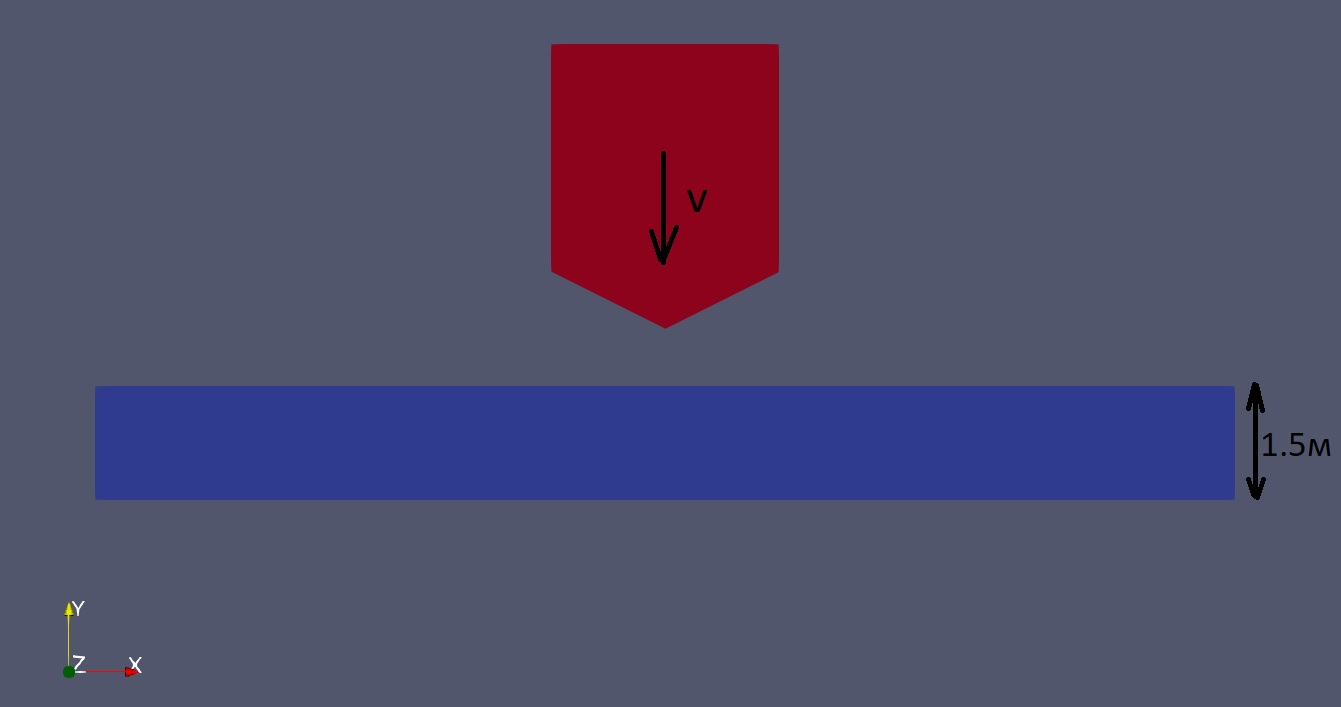
\includegraphics[width=1\linewidth]{task_ship.jpg} \\ (a) Острый нос}
\end{minipage}
\hfill
\begin{minipage}[h]{0.5\linewidth}
\center{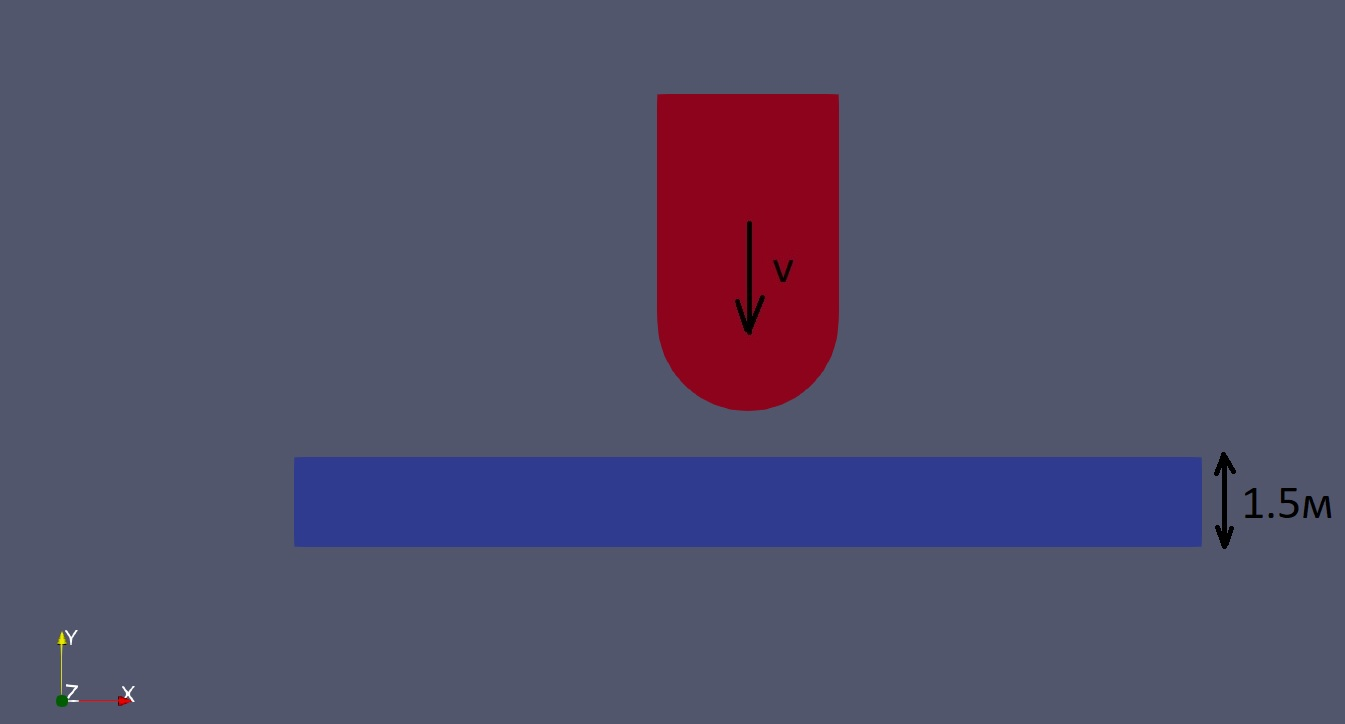
\includegraphics[width=1\linewidth]{task_circle_ship.jpg} \\ (b) Скругленный нос}
\end{minipage}
\caption{Постановка двумерной задачи}
\label{ris:image1}
\end{figure}
\par
На всевозможных граничных ячейках было задано условие свободной границы. Между внутренными ячейками льда и налетающего тела использовалось полное слипание, а на контактной границе "лед-тело" использовалось свободное скольжение. 
\subsection{Результаты расчетов}

\section{Трехмерная задача}

\chapter{Руководство по использованию программы}

\chapter{Заключение}

\chapter{Список литературы}

\end{document}